\stopallthesefloats
\subsubsection{WCET analysis}
\begin{figure}[hbt]
\centering
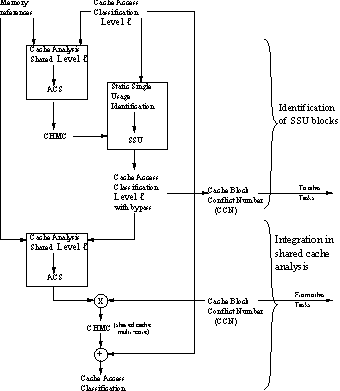
\includegraphics[width=0.65\columnwidth]{\chapterdirectory/figure/handling_it/bypass_to_wcet.pdf}
\caption{%
Overview of the strategy presented in \cite{10.1109/RTSS.2009.34} (taken
from the paper)
}
\label{fig:handling_it:bypass_to_wcet}
\end{figure}

\cite{10.1109/RTSS.2009.34} proposes a way to compute WCET for multi-core
architectures, with considerations for shared instruction caches with multiple
levels of hierarchy. It also tries out a \textit{bypassing scheme}, which
relies on the identification of single-use program blocks within shared
instruction caches to compile programs in a way that reduces interference
between tasks.

The proposed WCET computation strategy is based on existing approaches for
multi-levels instruction caches in single core processors. It uses static
analysis to categorizes all accesses as either: always-miss, always-hit,
first-miss (first access is unknown, but all following accesses will hit), and
not classified (for accesses that fail to be categorized in the other
patterns). This categorization (referred to as \textit{CHMC} in the paper) is
done for every cache level. Furthermore, the likeliness of an access actually
reaching a level is also evaluated and categorized with similar labels (always
acceded, never, always after the first access, unknown). Moving this strategy
to multi-core processors is indicated as having the potential of changing some
always-hit and first-miss into first-miss and \textit{not classified}. Accesses
made by different tasks on the same level where the categorization indicates
that the access is not \textit{never} done are considered as interfering with
one another (regardless of when the accesses are made). This is then used to
re-evaluate the hit/miss categorization so that it has the interference taken
into account. The result of the interference identification analysis is referred
to as \textit{C}ache block \textit{C}onflict \textit{N}umber. To improve the
precision of the result, the possibility of having code shared among tasks
(such as libraries) is taken into account. An overview of the whole process for
a given cache level $\ell$ is shown in
Figure~\ref{fig:handling_it:bypass_to_wcet}.

The decisions made in what to cache generally follow the
locality of reference principle, where the proximity of elements in memory is
assumed to translate to a proximity is usage times, and that processors
receptively access the same elements within short time periods. In
\cite{10.1109/RTSS.2009.34}, static analysis is used to find elements which are
only used once (called \textit{S}tatic \textit{S}ingle \textit{U}sage), in
order to avoid having them pollute caches and risk being considered as a source
of interference needlessly. This relies on a bypass mechanism, that allows
fetching data without altering the caches: if it is not found within any cache,
the value is retrieved but not added to any cache; if it is found within a
cache, the caches in-between do not get any copy, and the copy that was used is
not updated to indicate a recent access.
\stopallthesefloats
